\documentclass[12pt,a4paper,oneside,openany]{memoir}

\usepackage[utf8]{inputenc}
\usepackage[frenchb]{babel}
\usepackage[T1]{fontenc}

% Paquets utiles
\usepackage{graphicx}
\usepackage[usenames,svgnames]{xcolor}
\usepackage{tikz}
\usepackage{asymptote}
\usepackage{flafter}
\usepackage{multirow}
\usepackage{ifdraft}
%\usepackage[pdfpagelabels,draft,implicit=false]{hyperref}

%Tkiz
\usetikzlibrary{calc}
\usetikzlibrary{arrows}


% Décoration
\usepackage[lighttt]{lmodern} % pour le tt


% POUR MATHDESIGN : restaurer hrulefill
\let\xhrf\hrulefill
\usepackage[utopia]{mathdesign}
\let\hrulefill\xhrf
\renewcommand*{\chapterheadstart}{\begingroup
	\vspace*{\beforechapskip}%
	\begin{adjustwidth}{}{-\chapindent}%
		\hrulefill
		\smash{\rule{0.4pt}{15mm}}
	\end{adjustwidth}\endgroup}
%\usepackage{tgpagella}
\let\mathbb\relax \usepackage{bbold}
\fixpdflayout
%\counterwithout{section}{chapter}
%\setsecnumdepth{subsection}


\chapterstyle{ell}
\setsecheadstyle{\Large\bfseries\sffamily\raggedright}
\setsubsecheadstyle{\large\bfseries\sffamily\raggedright}
\midsloppy

\makepagestyle{myruled}
\makeoddfoot{myruled}{}{\thepage}{}
\makeevenfoot{myruled}{}{\thepage}{}
\makeheadrule{myruled}{\textwidth}{\normalrulethickness}
\makeevenhead{myruled}{\rightmark}{}{}
\makeoddhead{myruled}{\rightmark}{}{}
\pagestyle{myruled}

\captiondelim{ : }
\captiontitlefont{\sffamily}

\newsubfloat{figure}
\newsubfloat{table}

\newcommand{\anonchapter}[1]{\chapter*{#1}\addcontentsline{toc}{chapter}{\numberline{}#1}}
\newcommand{\todo}[1]{\marginpar{\textcolor{red}{#1}}}
\newcommand{\fltbrule}{\hrule\vspace{\onelineskip}}
\newcommand{\fltarule}{\vspace{\onelineskip}
	\hrule\vspace{\onelineskip}}

\author{Charles Bine\\Matthieu Félix}
\title{\\Production d'énergie électrique (centrales nucléaires et barrages hydroélectriques)}
\date{Décembre 2015}


% EXEMPLES & référence rapide
% dessin asymptote
% \lstinputlisting[firstline=, lastline=]{fichier}

\begin{document}
	
% Page de titre
\keepthetitle
\begin{titlingpage}
\noindent
\begin{minipage}[t]{0.5\textwidth} \begin{flushleft}
\theauthor \\ \thedate
\end{flushleft} \end{minipage}
\begin{minipage}[t]{0.5\textwidth} \begin{flushright}
Rapport de projet \\
Cours de réseaux électriques
\end{flushright} \end{minipage}

\vspace{3cm}
\begin{center}
{\LARGE \textbf{\thetitle}}
\ifdraft{\par Brouillon}{}
\end{center}
\vspace{3cm}

\end{titlingpage}

\addtolength{\marginparwidth}{11mm}
\abnormalparskip{4mm}

\clearpage

\tableofcontents

\clearpage

\chapter{Aperçu de la production d'énergie électrique}


\chapter{Le turbo-alternateur, au cœur de la production d'énergie électrique}

\begin{figure}
\centering
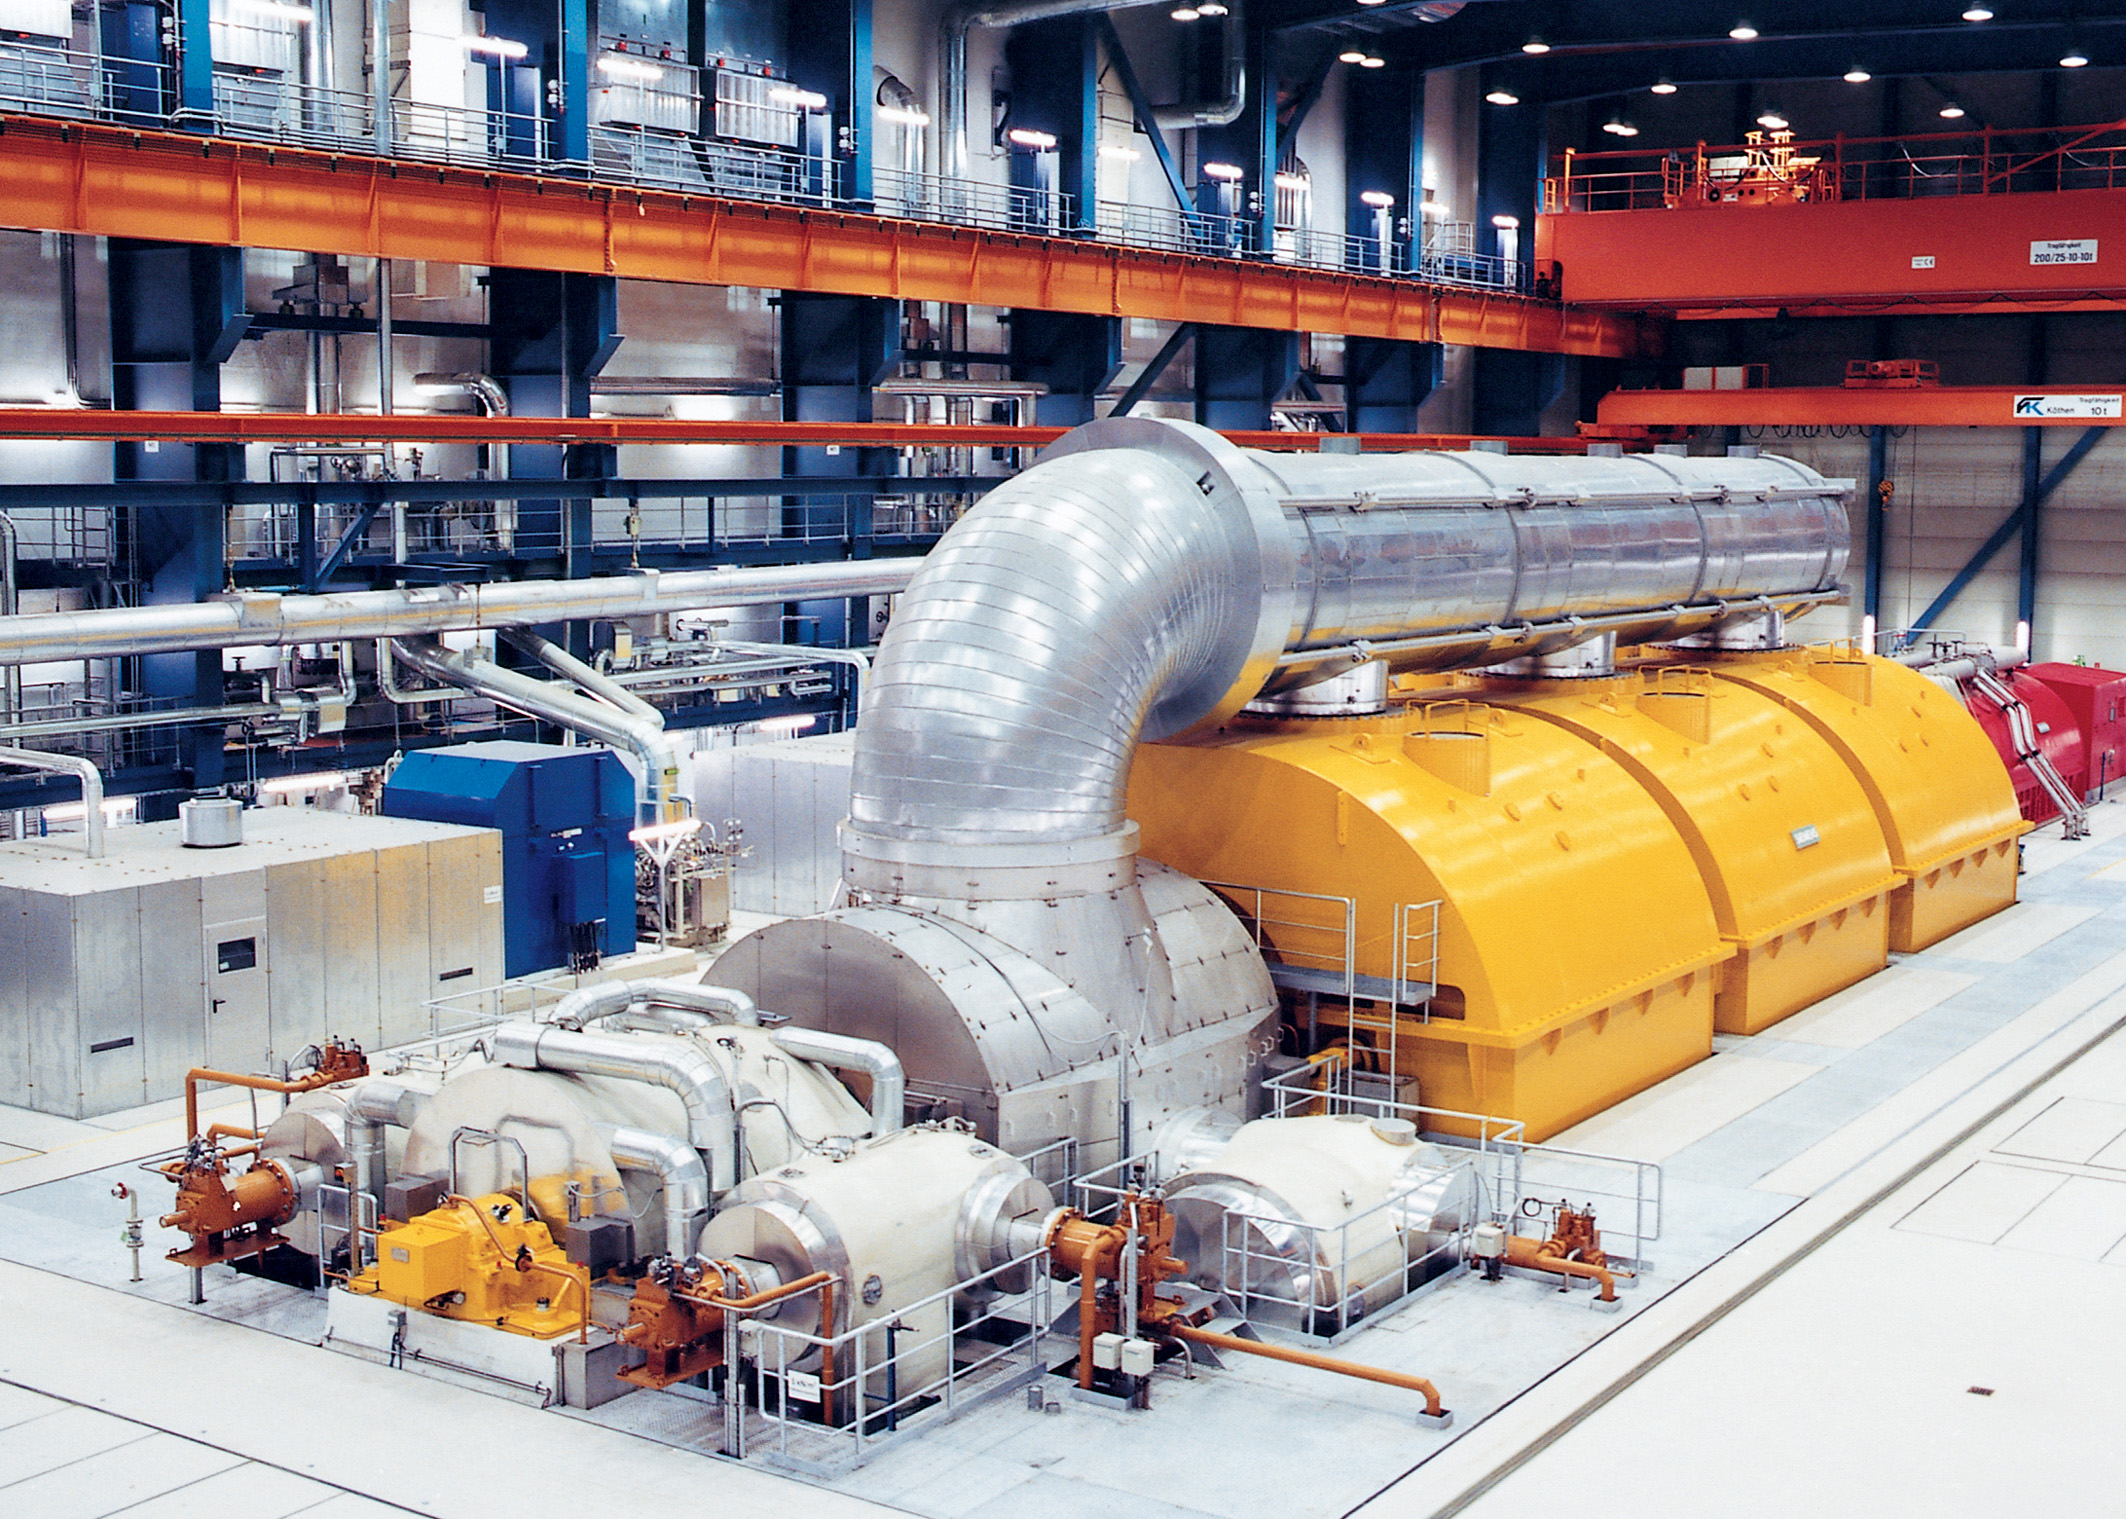
\includegraphics[width=0.95\linewidth]{Turbogenerator01}
\caption{Un turbo-alternateur moderne}
\label{fig:turbogenerator}
\end{figure}

\begin{figure}
\centering
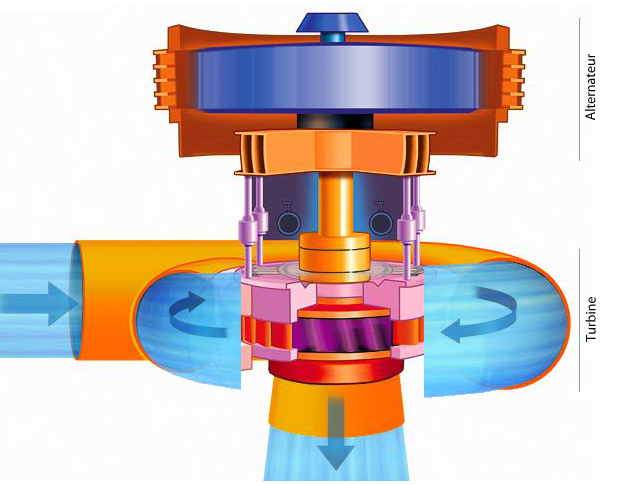
\includegraphics[width=0.9\linewidth]{coupe_turbo_alternateur}
\caption{Un turbo-alternateur à eau vu en coupe}
\label{fig:coupe_turbo_alternateur}
\end{figure}

De nombreux types de centrales modernes (à gaz, à charbon, hydro-électriques, nucléaires,\textellipsis) fonctionnent à l'aide de \emph{turbo-alternateurs} : une association entre une turbine et un alternateur.

\section{Turbine}

\section{Alternateur}
L'alternateur permet de convertir un mouvement mécanique de rotation, fourni par la turbine, en un courant électrique alternatif généralement triphasé.

L'alternateur fonctionne avec un rotor et un stator. Le rotor est entraîné par la turbine et est composé d'une série d'électroaimants ; le stator est fixé au bâti, et est recouvert de bobines dans lesquelles le courant sera induit.

Le bobinage de cette partie s'effectue comme celui des machines à courant alternatif, décrit dans le cours. On notera qu'il est assez fréquent que le bobinage du stator soit fait avec plus de deux pôles, ce qui permet de réduire la vitesse de rotation en conservant la fréquence du courant produit. Ainsi, les grandes centrales hydroélectriques utilisent généralement entre 16 et 64 pôles dans leurs alternateurs.

Le fait que les électroaimants soient situés sur le rotor pose également un problème, puisqu'ils doivent être alimentés. Plutôt que d'utiliser des balais et une piste circulaire pour transmettre le courant, les grands turbo-alternateurs se composent en fait de deux alternateurs. L'alternateur secondaire est monté dans la configuration inverse, c'est à dire que les aimants sont montés sur le stator et le bobinage passif est monté sur le rotor. Le courant ainsi produit sur le rotor est redressé, puis utilisé pour alimenter les électroaimants.

On notera aussi que l'intensité du courant dans les électroaimants de l'alternateur principale peut être modifiée pour adapter le courant produit par celui-ci : un courant plus grand dans les électroaimants induira un courant produit plus grand, mais une vitesse de rotation plus faible.


\subsection{Refroidissement}
Le refroidissement des alternateurs est un problème important puisque ceux-ci tournent souvent en continu (particulièrement dans le cas des centrales nucléaires) et à de fortes charges. Le refroidissement des alternateurs se fait couramment à l'aide d'hydrogène, produit dans les centrales par électrolyse et que l'on fait circuler entre le rotor et le stator. Cet hydrogène est ensuite refroidi dans un échangeur thermique avec de l'eau.

Cette solution relativement peu onéreuse (même s'il convient alors de faire très attention à l'étanchéité de l'alternateur) permet d'obtenir de très hautes disponibilités des turbo-alternateurs.


\section{Synchronisation}



\chapter{La centrale nucléaire}


\chapter{Le barrage hydroélectrique}


\end{document}
